\subsubsection{Admin Viewer}
A user is requested to enter a password before they are granted access to Admin
Viewer. The interface was implemented in the following manner:
\begin{description}
\item[Entity Chooser] This was implemented as EntityPopup, a PopupPanel with a
SuggestBox which allows the user to choose which type of entity to view. It
then requests it from the Datastore and directs the user to the DataViewer.
\item[Entity Viewer]This was implemented as DataViewer which provides the user
with a tabular view of all the entities of a particular type. It provides links
to EntityPopup and EditPopup.
\item[Entity Editor] This was implemented as EditPopup, a PopupPanel wich allows
a user to edit the various fields of a single entity or delete it completely.
After deleting or editing an entity, the DataViewer is updated with the new data
from the Datastore.
\end{description}
\begin{figure}[h!]
\centering
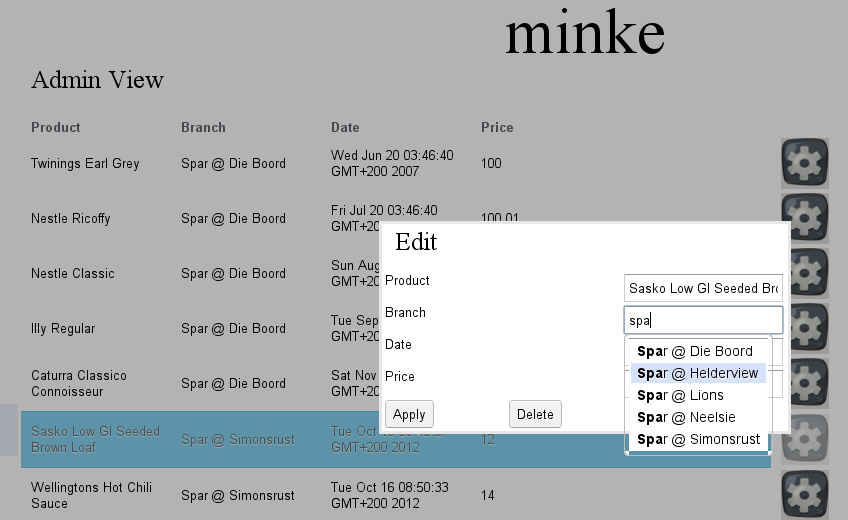
\includegraphics[width=0.8\textwidth]{gwt-admin.png}
\caption{The Entity Editor with Entity Viewer in the background.}
\end{figure}
